
\documentclass[conference]{../sty/llncs}
% Add the compsoc option for Computer Society conferences.
%
% If IEEEtran.cls has not been installed into the LaTeX system files,
% manually specify the path to it like:
% \documentclass[conference]{../sty/IEEEtran}
\usepackage{makeidx}
\usepackage{graphicx}
\usepackage{float}
\usepackage{url}
%\usepackage{caption}

% Some very useful LaTeX packages include:
% (uncomment the ones you want to load)


% *** MISC UTILITY PACKAGES ***
%
%\usepackage{ifpdf}
% Heiko Oberdiek's ifpdf.sty is very useful if you need conditional
% compilation based on whether the output is pdf or dvi.
% usage:
% \ifpdf
%   % pdf code
% \else
%   % dvi code
% \fi
% The latest version of ifpdf.sty can be obtained from:
% http://www.ctan.org/tex-archive/macros/latex/contrib/oberdiek/
% Also, note that IEEEtran.cls V1.7 and later provides a builtin
% \ifCLASSINFOpdf conditional that works the same way.
% When switching from latex to pdflatex and vice-versa, the compiler may
% have to be run twice to clear warning/error messages.






% *** CITATION PACKAGES ***
%
%\usepackage{cite}
% cite.sty was written by Donald Arseneau
% V1.6 and later of IEEEtran pre-defines the format of the cite.sty package
% \cite{} output to follow that of IEEE. Loading the cite package will
% result in citation numbers being automatically sorted and properly
% "compressed/ranged". e.g., [1], [9], [2], [7], [5], [6] without using
% cite.sty will become [1], [2], [5]--[7], [9] using cite.sty. cite.sty's
% \cite will automatically add leading space, if needed. Use cite.sty's
% noadjust option (cite.sty V3.8 and later) if you want to turn this off.
% cite.sty is already installed on most LaTeX systems. Be sure and use
% version 4.0 (2003-05-27) and later if using hyperref.sty. cite.sty does
% not currently provide for hyperlinked citations.
% The latest version can be obtained at:
% http://www.ctan.org/tex-archive/macros/latex/contrib/cite/
% The documentation is contained in the cite.sty file itself.






% *** GRAPHICS RELATED PACKAGES ***
%
%\ifCLASSINFOpdf
  % \usepackage[pdftex]{graphicx}
  % declare the path(s) where your graphic files are
  % \graphicspath{{../pdf/}{../jpeg/}}
  % and their extensions so you won't have to specify these with
  % every instance of \includegraphics
  % \DeclareGraphicsExtensions{.pdf,.jpeg,.png}
%\else
  % or other class option (dvipsone, dvipdf, if not using dvips). graphicx
  % will default to the driver specified in the system graphics.cfg if no
  % driver is specified.
  % \usepackage[dvips]{graphicx}
  % declare the path(s) where your graphic files are
  % \graphicspath{{../eps/}}
  % and their extensions so you won't have to specify these with
  % every instance of \includegraphics
  % \DeclareGraphicsExtensions{.eps}
%\fi
% graphicx was written by David Carlisle and Sebastian Rahtz. It is
% required if you want graphics, photos, etc. graphicx.sty is already
% installed on most LaTeX systems. The latest version and documentation can
% be obtained at: 
% http://www.ctan.org/tex-archive/macros/latex/required/graphics/
% Another good source of documentation is "Using Imported Graphics in
% LaTeX2e" by Keith Reckdahl which can be found as epslatex.ps or
% epslatex.pdf at: http://www.ctan.org/tex-archive/info/
%
% latex, and pdflatex in dvi mode, support graphics in encapsulated
% postscript (.eps) format. pdflatex in pdf mode supports graphics
% in .pdf, .jpeg, .png and .mps (metapost) formats. Users should ensure
% that all non-photo figures use a vector format (.eps, .pdf, .mps) and
% not a bitmapped formats (.jpeg, .png). IEEE frowns on bitmapped formats
% which can result in "jaggedy"/blurry rendering of lines and letters as
% well as large increases in file sizes.
%
% You can find documentation about the pdfTeX application at:
% http://www.tug.org/applications/pdftex





% *** MATH PACKAGES ***
%
%\usepackage[cmex10]{amsmath}
% A popular package from the American Mathematical Society that provides
% many useful and powerful commands for dealing with mathematics. If using
% it, be sure to load this package with the cmex10 option to ensure that
% only type 1 fonts will utilized at all point sizes. Without this option,
% it is possible that some math symbols, particularly those within
% footnotes, will be rendered in bitmap form which will result in a
% document that can not be IEEE Xplore compliant!
%
% Also, note that the amsmath package sets \interdisplaylinepenalty to 10000
% thus preventing page breaks from occurring within multiline equations. Use:
%\interdisplaylinepenalty=2500
% after loading amsmath to restore such page breaks as IEEEtran.cls normally
% does. amsmath.sty is already installed on most LaTeX systems. The latest
% version and documentation can be obtained at:
% http://www.ctan.org/tex-archive/macros/latex/required/amslatex/math/





% *** SPECIALIZED LIST PACKAGES ***
%
%\usepackage{algorithmic}
% algorithmic.sty was written by Peter Williams and Rogerio Brito.
% This package provides an algorithmic environment fo describing algorithms.
% You can use the algorithmic environment in-text or within a figure
% environment to provide for a floating algorithm. Do NOT use the algorithm
% floating environment provided by algorithm.sty (by the same authors) or
% algorithm2e.sty (by Christophe Fiorio) as IEEE does not use dedicated
% algorithm float types and packages that provide these will not provide
% correct IEEE style captions. The latest version and documentation of
% algorithmic.sty can be obtained at:
% http://www.ctan.org/tex-archive/macros/latex/contrib/algorithms/
% There is also a support site at:
% http://algorithms.berlios.de/index.html
% Also of interest may be the (relatively newer and more customizable)
% algorithmicx.sty package by Szasz Janos:
% http://www.ctan.org/tex-archive/macros/latex/contrib/algorithmicx/




% *** ALIGNMENT PACKAGES ***
%
%\usepackage{array}
% Frank Mittelbach's and David Carlisle's array.sty patches and improves
% the standard LaTeX2e array and tabular environments to provide better
% appearance and additional user controls. As the default LaTeX2e table
% generation code is lacking to the point of almost being broken with
% respect to the quality of the end results, all users are strongly
% advised to use an enhanced (at the very least that provided by array.sty)
% set of table tools. array.sty is already installed on most systems. The
% latest version and documentation can be obtained at:
% http://www.ctan.org/tex-archive/macros/latex/required/tools/


%\usepackage{mdwmath}
%\usepackage{mdwtab}
% Also highly recommended is Mark Wooding's extremely powerful MDW tools,
% especially mdwmath.sty and mdwtab.sty which are used to format equations
% and tables, respectively. The MDWtools set is already installed on most
% LaTeX systems. The lastest version and documentation is available at:
% http://www.ctan.org/tex-archive/macros/latex/contrib/mdwtools/


% IEEEtran contains the IEEEeqnarray family of commands that can be used to
% generate multiline equations as well as matrices, tables, etc., of high
% quality.


%\usepackage{eqparbox}
% Also of notable interest is Scott Pakin's eqparbox package for creating
% (automatically sized) equal width boxes - aka "natural width parboxes".
% Available at:
% http://www.ctan.org/tex-archive/macros/latex/contrib/eqparbox/





% *** SUBFIGURE PACKAGES ***
%\usepackage[tight,footnotesize]{subfigure}
% subfigure.sty was written by Steven Douglas Cochran. This package makes it
% easy to put subfigures in your figures. e.g., "Figure 1a and 1b". For IEEE
% work, it is a good idea to load it with the tight package option to reduce
% the amount of white space around the subfigures. subfigure.sty is already
% installed on most LaTeX systems. The latest version and documentation can
% be obtained at:
% http://www.ctan.org/tex-archive/obsolete/macros/latex/contrib/subfigure/
% subfigure.sty has been superceeded by subfig.sty.



%\usepackage[caption=false]{caption}
%\usepackage[font=footnotesize]{subfig}
% subfig.sty, also written by Steven Douglas Cochran, is the modern
% replacement for subfigure.sty. However, subfig.sty requires and
% automatically loads Axel Sommerfeldt's caption.sty which will override
% IEEEtran.cls handling of captions and this will result in nonIEEE style
% figure/table captions. To prevent this problem, be sure and preload
% caption.sty with its "caption=false" package option. This is will preserve
% IEEEtran.cls handing of captions. Version 1.3 (2005/06/28) and later 
% (recommended due to many improvements over 1.2) of subfig.sty supports
% the caption=false option directly:
%\usepackage[caption=false,font=footnotesize]{subfig}
%
% The latest version and documentation can be obtained at:
% http://www.ctan.org/tex-archive/macros/latex/contrib/subfig/
% The latest version and documentation of caption.sty can be obtained at:
% http://www.ctan.org/tex-archive/macros/latex/contrib/caption/




% *** FLOAT PACKAGES ***
%
%\usepackage{fixltx2e}
% fixltx2e, the successor to the earlier fix2col.sty, was written by
% Frank Mittelbach and David Carlisle. This package corrects a few problems
% in the LaTeX2e kernel, the most notable of which is that in current
% LaTeX2e releases, the ordering of single and double column floats is not
% guaranteed to be preserved. Thus, an unpatched LaTeX2e can allow a
% single column figure to be placed prior to an earlier double column
% figure. The latest version and documentation can be found at:
% http://www.ctan.org/tex-archive/macros/latex/base/



%\usepackage{stfloats}
% stfloats.sty was written by Sigitas Tolusis. This package gives LaTeX2e
% the ability to do double column floats at the bottom of the page as well
% as the top. (e.g., "\begin{figure*}[!b]" is not normally possible in
% LaTeX2e). It also provides a command:
%\fnbelowfloat
% to enable the placement of footnotes below bottom floats (the standard
% LaTeX2e kernel puts them above bottom floats). This is an invasive package
% which rewrites many portions of the LaTeX2e float routines. It may not work
% with other packages that modify the LaTeX2e float routines. The latest
% version and documentation can be obtained at:
% http://www.ctan.org/tex-archive/macros/latex/contrib/sttools/
% Documentation is contained in the stfloats.sty comments as well as in the
% presfull.pdf file. Do not use the stfloats baselinefloat ability as IEEE
% does not allow \baselineskip to stretch. Authors submitting work to the
% IEEE should note that IEEE rarely uses double column equations and
% that authors should try to avoid such use. Do not be tempted to use the
% cuted.sty or midfloat.sty packages (also by Sigitas Tolusis) as IEEE does
% not format its papers in such ways.





% *** PDF, URL AND HYPERLINK PACKAGES ***
%
%\usepackage{url}
% url.sty was written by Donald Arseneau. It provides better support for
% handling and breaking URLs. url.sty is already installed on most LaTeX
% systems. The latest version can be obtained at:
% http://www.ctan.org/tex-archive/macros/latex/contrib/misc/
% Read the url.sty source comments for usage information. Basically,
% \url{my_url_here}.





% *** Do not adjust lengths that control margins, column widths, etc. ***
% *** Do not use packages that alter fonts (such as pslatex).         ***
% There should be no need to do such things with IEEEtran.cls V1.6 and later.
% (Unless specifically asked to do so by the journal or conference you plan
% to submit to, of course. )


% correct bad hyphenation here
\hyphenation{op-tical net-works semi-conduc-tor}


\begin{document}
%
% paper title
% can use linebreaks \\ within to get better formatting as desired
\title{Real-Time Prediction of Blood Alcohol Content using Smartwatch Sensor Data}


% author names and affiliations
% use a multiple column layout for up to three different
% affiliations
\author{Mario A. Gutierrez \and Michelle L. Fast \and Anne H. Ngu \and  Byron J. Gao}
\institute{Department of Computer Science, Texas State University, San Marcos, Texas, USA\\
\email{\{mag262|mlf96|angu|bgao\}@txstate.edu}
}
%\author{
%	\IEEEauthorblockN{Mario A. Gutierrez}
%	\IEEEauthorblockA{mag262@txstate.edu}
%\and
%	\IEEEauthorblockN{Michelle L. Fast}
%	\IEEEauthorblockA{mlf96@txstate.edu}
%\and
	%\IEEEauthorblockN{Anne H. Ngu}
	%\IEEEauthorblockA{angu@txstate.edu}
%\and
	%\IEEEauthorblockN{Byron Gao}
	%\IEEEauthorblockA{bgao@txstate.edu}
%}

% conference papers do not typically use \thanks and this command
% is locked out in conference mode. If really needed, such as for
% the acknowledgment of grants, issue a \IEEEoverridecommandlockouts
% after \documentclass

% for over three affiliations, or if they all won't fit within the width
% of the page, use this alternative format:
% 
%\author{\IEEEauthorblockN{Michael Shell\IEEEauthorrefmark{1},
%Homer Simpson\IEEEauthorrefmark{2},
%James Kirk\IEEEauthorrefmark{3}, 
%Montgomery Scott\IEEEauthorrefmark{3} and
%Eldon Tyrell\IEEEauthorrefmark{4}}
%\IEEEauthorblockA{\IEEEauthorrefmark{1}School of Electrical and Computer Engineering\\
%Georgia Institute of Technology,
%Atlanta, Georgia 30332--0250\\ Email: see http://www.michaelshell.org/contact.html}
%\IEEEauthorblockA{\IEEEauthorrefmark{2}Twentieth Century Fox, Springfield, USA\\
%Email: homer@thesimpsons.com}
%\IEEEauthorblockA{\IEEEauthorrefmark{3}Starfleet Academy, San Francisco, California 96678-2391\\
%Telephone: (800) 555--1212, Fax: (888) 555--1212}
%\IEEEauthorblockA{\IEEEauthorrefmark{4}Tyrell Inc., 123 Replicant Street, Los Angeles, California 90210--4321}}




% use for special paper notices
%\IEEEspecialpapernotice{(Invited Paper)}




% make the title area
\maketitle

\begin{abstract}
This paper proposes an application that collects sensor data from a smartwatch in order to predict drunkenness in real-time, discreetly, and non-invasively via a machine learning approach. This system could prevent drunk driving or other dangers related to the consumption of alcohol by giving users a way to determine personal intoxication level without the use of intrusive breathalyzers or guess work.  Using smartwatch data collected from several volunteers, we trained a machine learning model that may work with a smartphone application to predict the user's intoxication level in real-time.
\end{abstract}

%\begin{IEEEkeywords}
	%\lowercase{Sensor systems and applications, Temperature sensors, Machine learning, Prediction methods, Prediction algorithms, Internet of Things, Middleware, Wireless sensor networks}
%\end{IEEEkeywords}
\section{Introduction}
%% Domain introduction, problem, contributions, and organization of the paper.

Internet of Things (IoT) is a domain that represents the next most exciting technological revolution since the Internet. IoT will bring endless opportunities and impact every corner of our planet. In the healthcare domain, IoT promises to bring personalized health tracking and monitoring ever closer to the consumers. This phenomena is discussed in a recent Wall Street Journal article, "Why Connected Medicine Is Becoming Vital to Health Care" \cite{Landro:2015}. Modern smartphones and smartwatches now contain a more diverse collection of sensors than ever before, and people are warming up to them. In January 2014, approximately 46 million US smartphone owners were reported to have used health and fitness applications \cite{Nielsen:2014}. Currently, sports and fitness are the predominant foci of IoT-based health applications. However, applications in disease management and health care are becoming increasingly prevalent. For example, detecting falling of elderly patients \cite{Tacconi:2011}. 

Drunk driving is a dangerous, worldwide problem. This problem is not only a hazard to the drunk drivers, but also to pedestrians and other drivers. It is reported by the Bureau of Transportation Statistics that in 2010, 47.2\% of pedestrian fatalities and 39.9\% of vehicle occupant fatalities were caused by drunk driving \cite{Chambers:2012}. The Centers for Disease Control and Prevention (CDC) reported that between the years 2008 and 2010, roughly two-thirds of adults were drinkers, with adults between the ages 18 and 24 having the greatest association with heavy drinking \cite{Schoenborn:2013}. 

At dangerous levels of intoxication, it can be difficult to judge ones own drunkenness. Instead it would be better to get a definitive measurement of the BAC, or simply a binary response: "drunk" or "not drunk." Compact breathalyzers are probably the best option at the moment, but these are not discreet and require deliberate action by the user. The other option is to use a smartphone application to manually calculate BAC, but these demand a greater deal of involvement from the user. To be practical, it would be useful to have some sort of non-invasive and accurate monitoring system that will warn its user if they become too intoxicated. It has been shown that electronic intervention programs are more successful at reducing college student drinking than a general alcohol awareness program \cite{Ward:2015}. This system can also be used to warn friends and family, or prevent the operation of the user's car.

The main contributions of our paper are: \begin{itemize}
	\item A machine learning model for the prediction of intoxication level from smartwatch sensor data.
	\item A general Android-based gateway system that can collect data from any type of physical or virtual sensor accessible by the host smartphone.
\end{itemize}

%****Summary****
\section{Related Work}
%
%Include the current IoT middleware systems that you have surveyed. Should start this early.
%\input{related_work}

There is much research being done in the prediction or calculation of blood alcohol content. 

The most common way to calculate BAC is through the Widmark equation. Posey and Mozayani in their paper \cite{Posey:2007} discuss the Widmark equation and improvements on its use by observing 5 previously published models and one new model for BAC prediction. The Widmark equation predicts BAC using elimination rates and the Widmark factor. Current use of the Widmark equation and BAC prediction is discouraged by experts due to inaccuracies, usually overestimation. Mathematical calculation of BAC is still sometimes used in DUI court cases, as there are not many alternatives, but it requires lab test results, information about what the person was drinking, how much and how long, BMI, and other hard to find details such as elimination rates. Some of this information has to be estimated or generalized which causes the calculation to be inaccurate. Also, due to the amount of information required, such a method is unusable by the general public for personal use. While BAC prediction is generally frowned upon in court cases, Posey and Mozayani make a point that using several different models provides a more accurate prediction than using the original Widmark equation alone.

Another known method of measuring BAC is through a transdermal ethanol sensor. Webster and Gabler \cite{Webster:2007} discussed the feasibility of transdermal ethanol sensors being integrated into ignition interlock systems in order to prevent drunk driving. A way to reduce the number of incidents related to drunk driving is to somehow stop people from driving drunk. Their approach to do this is to fit every vehicle with a ignition interlock system that responds to the driver's BAC. Current interlock systems like this involve a breathalyzer, but these are seen as expensive, bulky, and elicit a negative response from the general public. Transdermal ethanol sensing provides a more discreet way to measure BAC. However, according to the paper, an issue with transdermal ethanol sensing is that there is a significant delay, up to roughly an hour, from the time of alcohol consumption and detection at the skin. 

In 2014, James Baldwin applied for a patent on a wearable blood alcohol measuring device \cite{Baldwin:2014} as a non-invasive, discreet, and wearable method of continuously predicting blood alcohol content. Baldwin's method involves the use of a transdermal ethanol sensor and a method of predicting future BAC given the user's intended consumption. It is also meant to provide guidance for the user as to when to stop in order to be at a certain BAC by a previously specified time. Baldwin's invention is very similar to this project with the only major difference being that it uses a wearable transdermal ethanol sensor to directly measure BAC instead of using common sensors found in smartwatches and a prediction model, such as we do, in order to predict BAC. The use of a transdermal ethanol sensor is proven to have many issues, mostly in the delay between consumption and sensing \cite{Webster:2007}. Another issue is that it requires a special sensor that would only be used for this purpose. Our project improves on this issue by using a common device that many already own for various other reasons. Also, due to our approach for monitoring drunkenness, our method may provide more immediate predictions.  

In 2015, Koukiou and Anastassopoulos published a paper on using a neural network to identify drunkenness from thermal infrared imagery \cite{Koukiou:2015}. Different neural networks were trained on different parts of the face in order to determine which areas can be used to discriminated "a drunk from a sober person." Their findings showed that the forehead was the main feature to change thermal behavior from the consumption of alcohol. Later, the whole face was used to train a neural structure which showed high performance on discrimination. The results showed that the forehead and the nose are the areas of the face that were most prominent in drunk people. A neural networks was then trained on the forehead of only one person which was then used on other persons in order to determine those who were drunk. The results had a success rate of around 90\%. This study shows that there is a correlation between skin temperature and drunkenness, which is applicable to our research because of the skin temperature sensor found on many smartwatches. This project has many similar applications as our would, such as being able to be incorporated into ignition interlock systems or to give evidence to authorities about intoxication in investigations. However, this system may not be able to be used by people to determine their own drunkenness as it requires a thermal infrared camera to be focused on the users face in order to do so. This would be difficult to do discreetly or conveniently. 

There is also research going into using various sensors for health applications, many using a machine learning approach to do so. 

In "Multi-Sensor Fusion for Enhanced Contextual Awareness of Everyday Activites with Ubiquitous Devices" \cite{Guiry:2014}, the authors attempt to use the sensors in smartphones and smartwatches to identify various daily activities such as walking, running, cycling, sitting, etc. It also identified whether or not the user is indoors or outdoors. Collected data was then used to train 5 different machine learning algorithms: C4.5, CART, Na\"{\i}ve Bayes, Multi-Layer Perceptrons, and Support Vector Machines. Results showed promise, with one model for inside/outside classification being 100\% correct. This study shows that the use of multiple sensors improves classification accuracy. For our research, we may be able to improve BAC prediction by recognizing when the user is taking a drink. This research shows that machine learning models can be used to label collected sensor data to certain activities.

Study has been done in using accelerometers to detect seizures \cite{Milosevic:2014} and using smartphones and smartwatches to monitor Parkinson Disease \cite{Sharma:2014}. In research on the detection of seizures \cite{Milosevic:2014}, researches use accelerometers on each wrist and ankle and a machine learning model in order to detect epileptic convulsions. Results included detection of 19 out of 23 seizures that were longer than 30 seconds each, with only a false alarm rate of .39 per hour. SPARK, a proposed framework that uses smartphones and smartwatches to monitor for symptoms of Parkinson Disease \cite{Sharma:2014}, including speech analysis, facial tremors, dyskinesia, freezing of gait. SPARK is for users to have their body motions monitored for dyskinesia and freezing gait while also having the user read paragraphs for speech analysis or pointing the camera for facial analysis. SPARK will also provide recommendations to physicians based on the collected information, such as changes in medication. SPARK is still being tested in order to determine the usefulness of such a framework for those who would use it. It is noted that there are limitations to it in that many patients will not be able to adopt the technologies required for it. There are also many issues, such as sensor misplacement and log errors, that can be encountered. Both these project show a desire to create health-based monitoring applications. 

%Current list of applications on smart watch, and their novelty. Current Prediction of BAC and associated ML algorithms
\section{System Architecture}
A custom Android application (Figure \ref{app}) was designed to be used during the study. This application collected and locally stored sensor data from a Microsoft Band smartwatch in a CSV file. The following data was collected from the Microsoft Band:
\begin{itemize}
	\item Accelerometer
	\item Gyroscope
	\item Pace
	\item Speed
	\item Distance traveled
	\item Motion type (idle, walking, etc.)
	\item Heart rate
	\item Pedometer
	\item Skin temperature
	\item Ultraviolet level
	\item Contact (if smartwatch is on)
	\item Calories burned
\end{itemize}
Additional data continuously collected and stored in the CSV by the application included:
\begin{itemize}
	\item GPS coordinates from the smartphone 
	\item Button that was pressed whenever the user took a drink
	\item Input field used to periodically record the BAC measured by a separate breathalyzer.
\end{itemize} 

\begin{figure}[H]
	\centering
	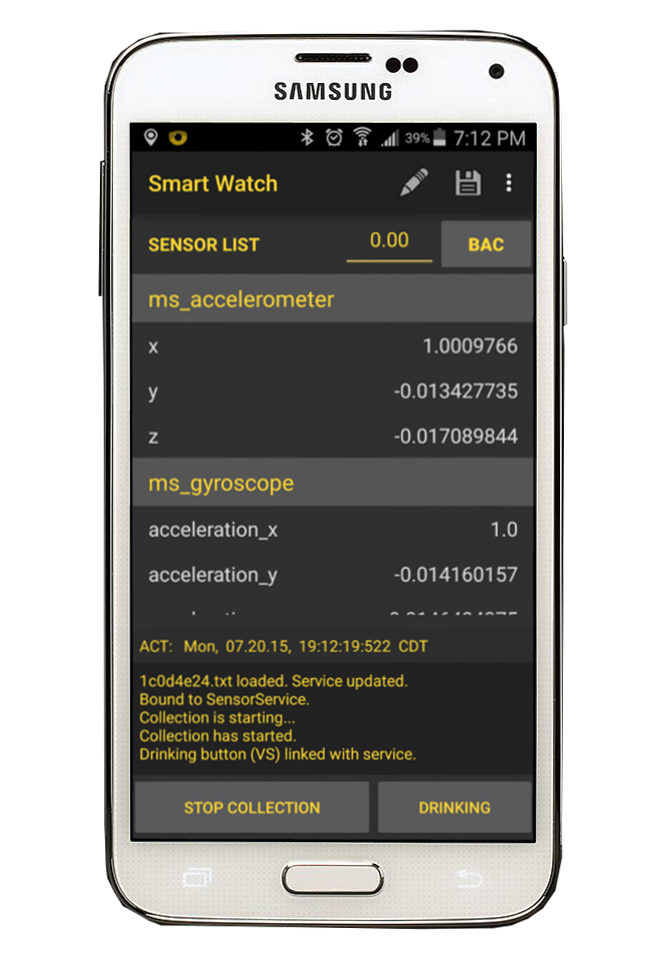
\includegraphics[scale=.20]{../figs/smartwatch.png}
	\caption{Capture of the Android application}
	\label{app}
\end{figure}

User information was also recorded and stored through the application before data collection began. Each user was given an unique user id (UUID) and the user profile included age, sex, body mass index, and blood type which was also stored locally as a JSON file.

After the data had been collected, the stored csv file and json file were uploaded to the web server and data inserted into mySQl database by a php script. Data stored on the MySQL database was then displayed on a web client by a geographical map. 

\begin{figure}[H]
	\centering
	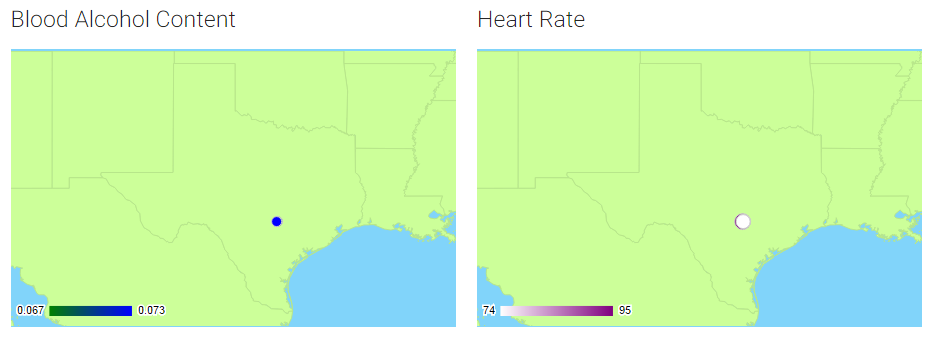
\includegraphics[scale=.35]{../figs/webpage.png}
	\caption{Current data visualization}
	\label{webpage}
\end{figure}

As of now, the web client displays the last sample for each user at the recorded location (Figure \ref{webpage}). Ideally in future systems, many samples will be averaged across regions (Figure \ref{concept}). 

\begin{figure}[H]
	\centering
	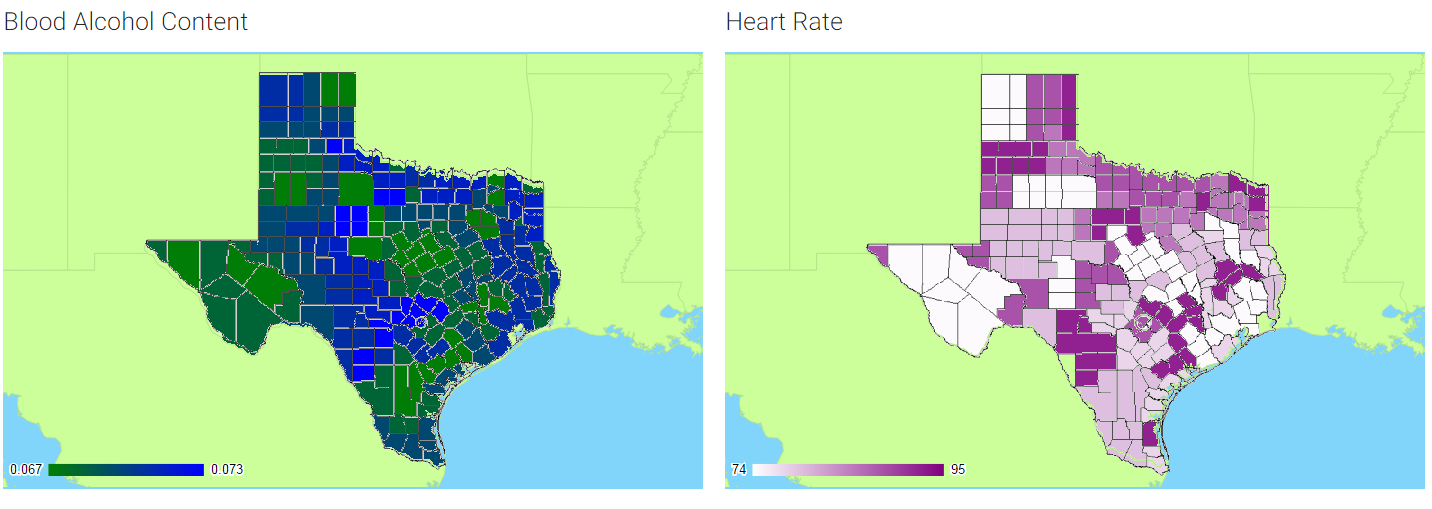
\includegraphics[scale=.23]{../figs/webconcept.png}
	\caption{Ideal data visualization}
	\label{concept}
\end{figure}

The collected data was also used to train a machine learning model which would be implemented in a future Android application to predict user BAC or drunkenness. 

\begin{figure}[H]
	\centering
	\includegraphics[scale=.30]{../figs/applicationsystem.png}
	\caption{Application system}
	\label{appsystem}
\end{figure}

Representation of this system can be found in Figure \ref{overallsystem}.

\begin{figure}[H]
	\centering
	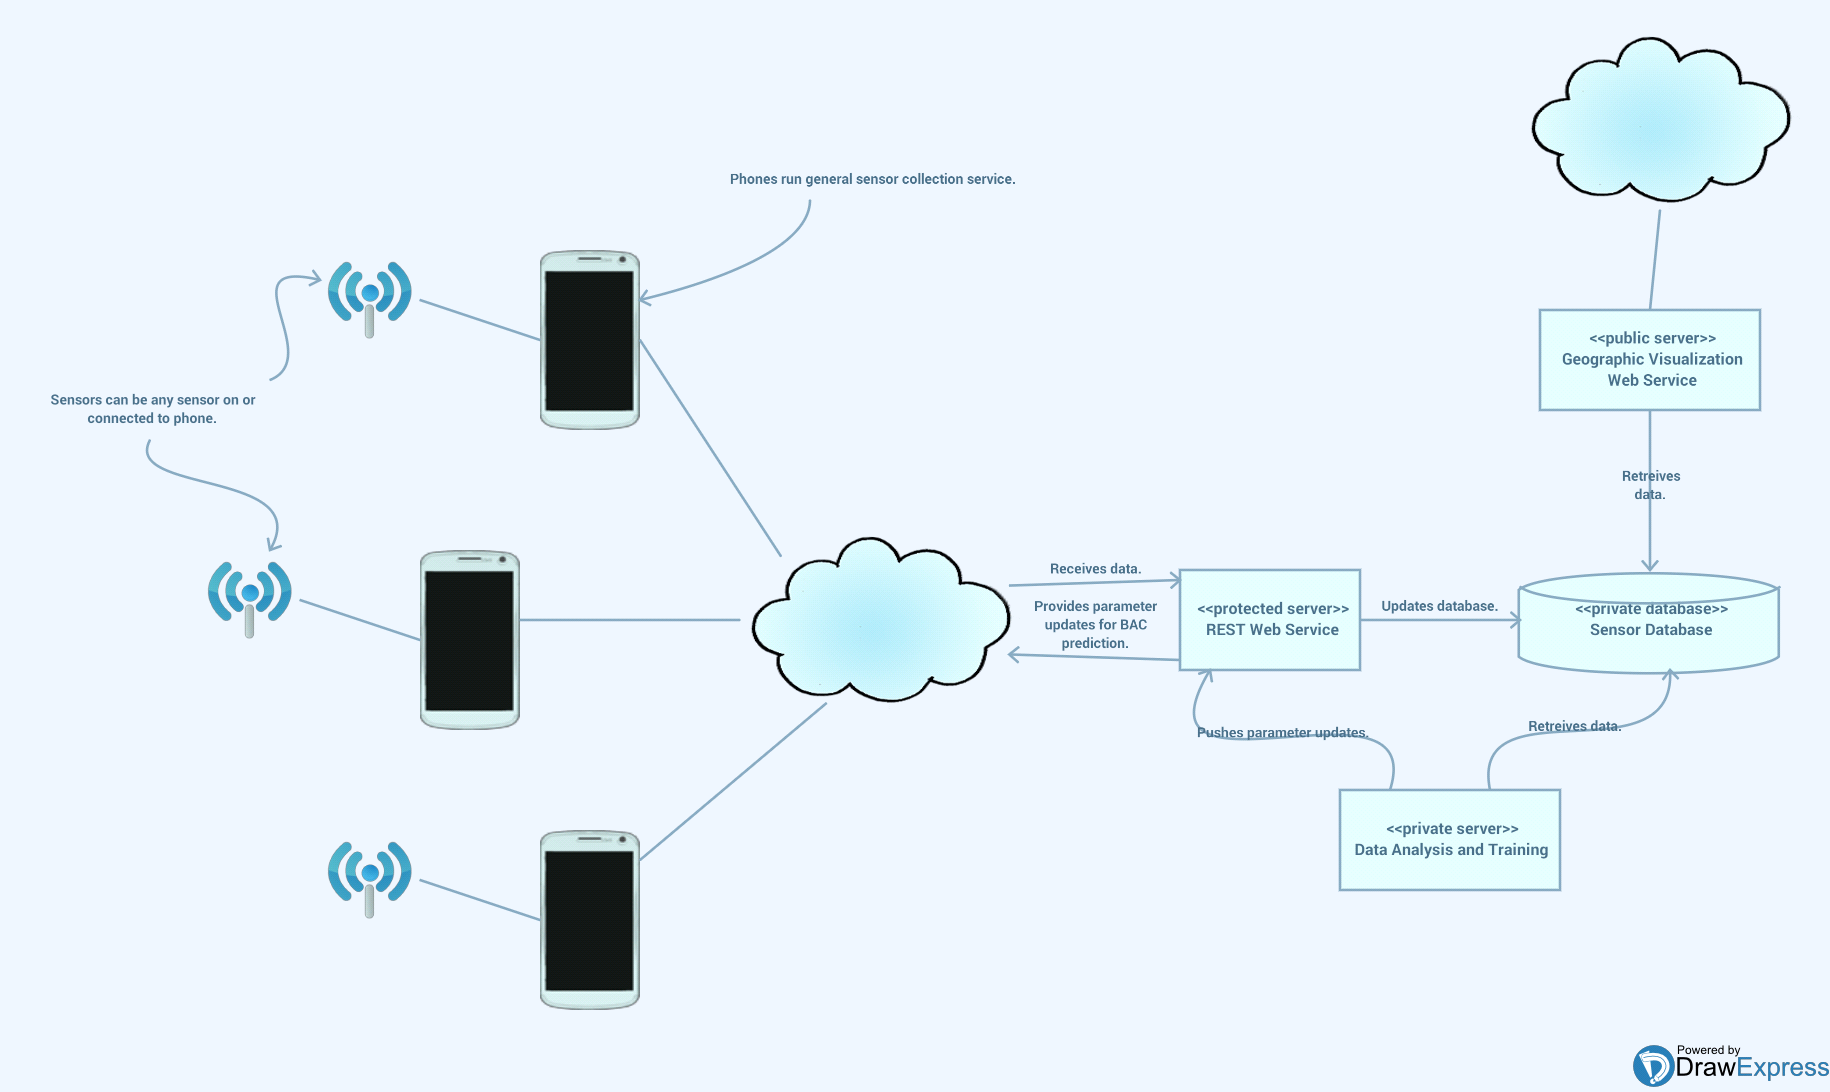
\includegraphics[scale=.14]{../figs/overall_system.png}
	\caption{Overall system}
	\label{overallsystem}
\end{figure}

\section{Methodology}

In this section, we will describe how we collected the data, we will present an analysis of the data, and then lead into the discussion of the machine learning models used.

\subsection{Collection}

Our collection began with the development of an Android application that connected to a Microsoft Band smartwatch and collected data from all of its available sensors. This development led to the general Android-based sensor gateway discussed in the previous section. Next, we developed a general procedure for our volunteers to follow during the collection of data. Our volunteers were eager to freely contribute the anonymous data used in this paper. The system collected the data into a .csv file on the Android smartphone and was also transmitted to a central MySQL server.

The Android platform was version 5.0 (kernel 3.4.0-4432708) running on a Samsung S5 smartphone. The Microsoft Band was Build Version 10.2.2818.0 09 R. Samples of the sensor data were collected every three seconds, based on the update speed of the Band's heart rate sensor. For every sample, the most recent sensor value was used for every sensor if available, else it would use the last updated value; or in the case of the accelerometer and gyroscope sensors, the last three values were averaged with linear weighting (the most recent having the most importance). There may be a better weighting, but this weighting was suitable for our purposes.

We designed a simple, two-hour procedure for the collection of the data. First, we established some necessary information about the subject to estimate the amount of alcohol necessary to reach 0.08 BAC in a 1.5 hour period using the Widmark equation (1). The particular formulation of it we used is the following: \begin{equation}
SD =  BW \cdot Wt \cdot (EBAC + (MR \cdot DP)) \cdot 0.4690
\end{equation} where $SD$ is the number of standard drinks (10 grams ethanol), $BW$ is the body water contant (0.58 for men and 0.49 for women), Wt is the body weight in lbs, EBAC is the estimated BAC, MR is the metabolism rate (0.17 for women and 0.18 for men), DP is the drinking period in hours, and  $0.4690 = 0.4536 \div (0.806 \cdot 1.2)$, a combination of two constants from the equation and a converstion from kg to lbs \cite{Andersson:2009}\cite{Wiki:BAC}. This amount was used to estimate the number of standard drinks to be consumed over the set time period, distributed over equal intervals. During this process, at every 25 minutes we took a measurement of the BAC using a BACtrack Trace\textsuperscript{TM} Pro breathalyzer. This measurement interval was determined by the cooldown rate of the breathalyzer. The activity chosen for the volunteers to engage in was a card or board game of their choice. Drinking stopped before 1.5 hours while collection and BAC measurement continued for another 30-45 minutes.

\subsection{Data Analysis}

The Microsoft Band we used has an assortment of interesting physical and virtual sensors that we can look at, including: an accelerometer, a gyroscope, distance, heart rate, pedometer, skin temperature, and ultraviolet level. With the sample size of five volunteers and a controlled setting for the experiments, some will not be as useful for this study: distance, pedometer, and ultraviolet level. In fact, their usefulness may be limited even with larger datasets. 

We begin our analysis with the heart rate (HR) by normalizing the heart rates and BACs per subject. This way we can plot and compare the HR values over the BAC and see if there are any obvious patterns. Doing this we get the plots shown in Figure \ref{fig:heart_rate_facet}.

\begin{figure}
	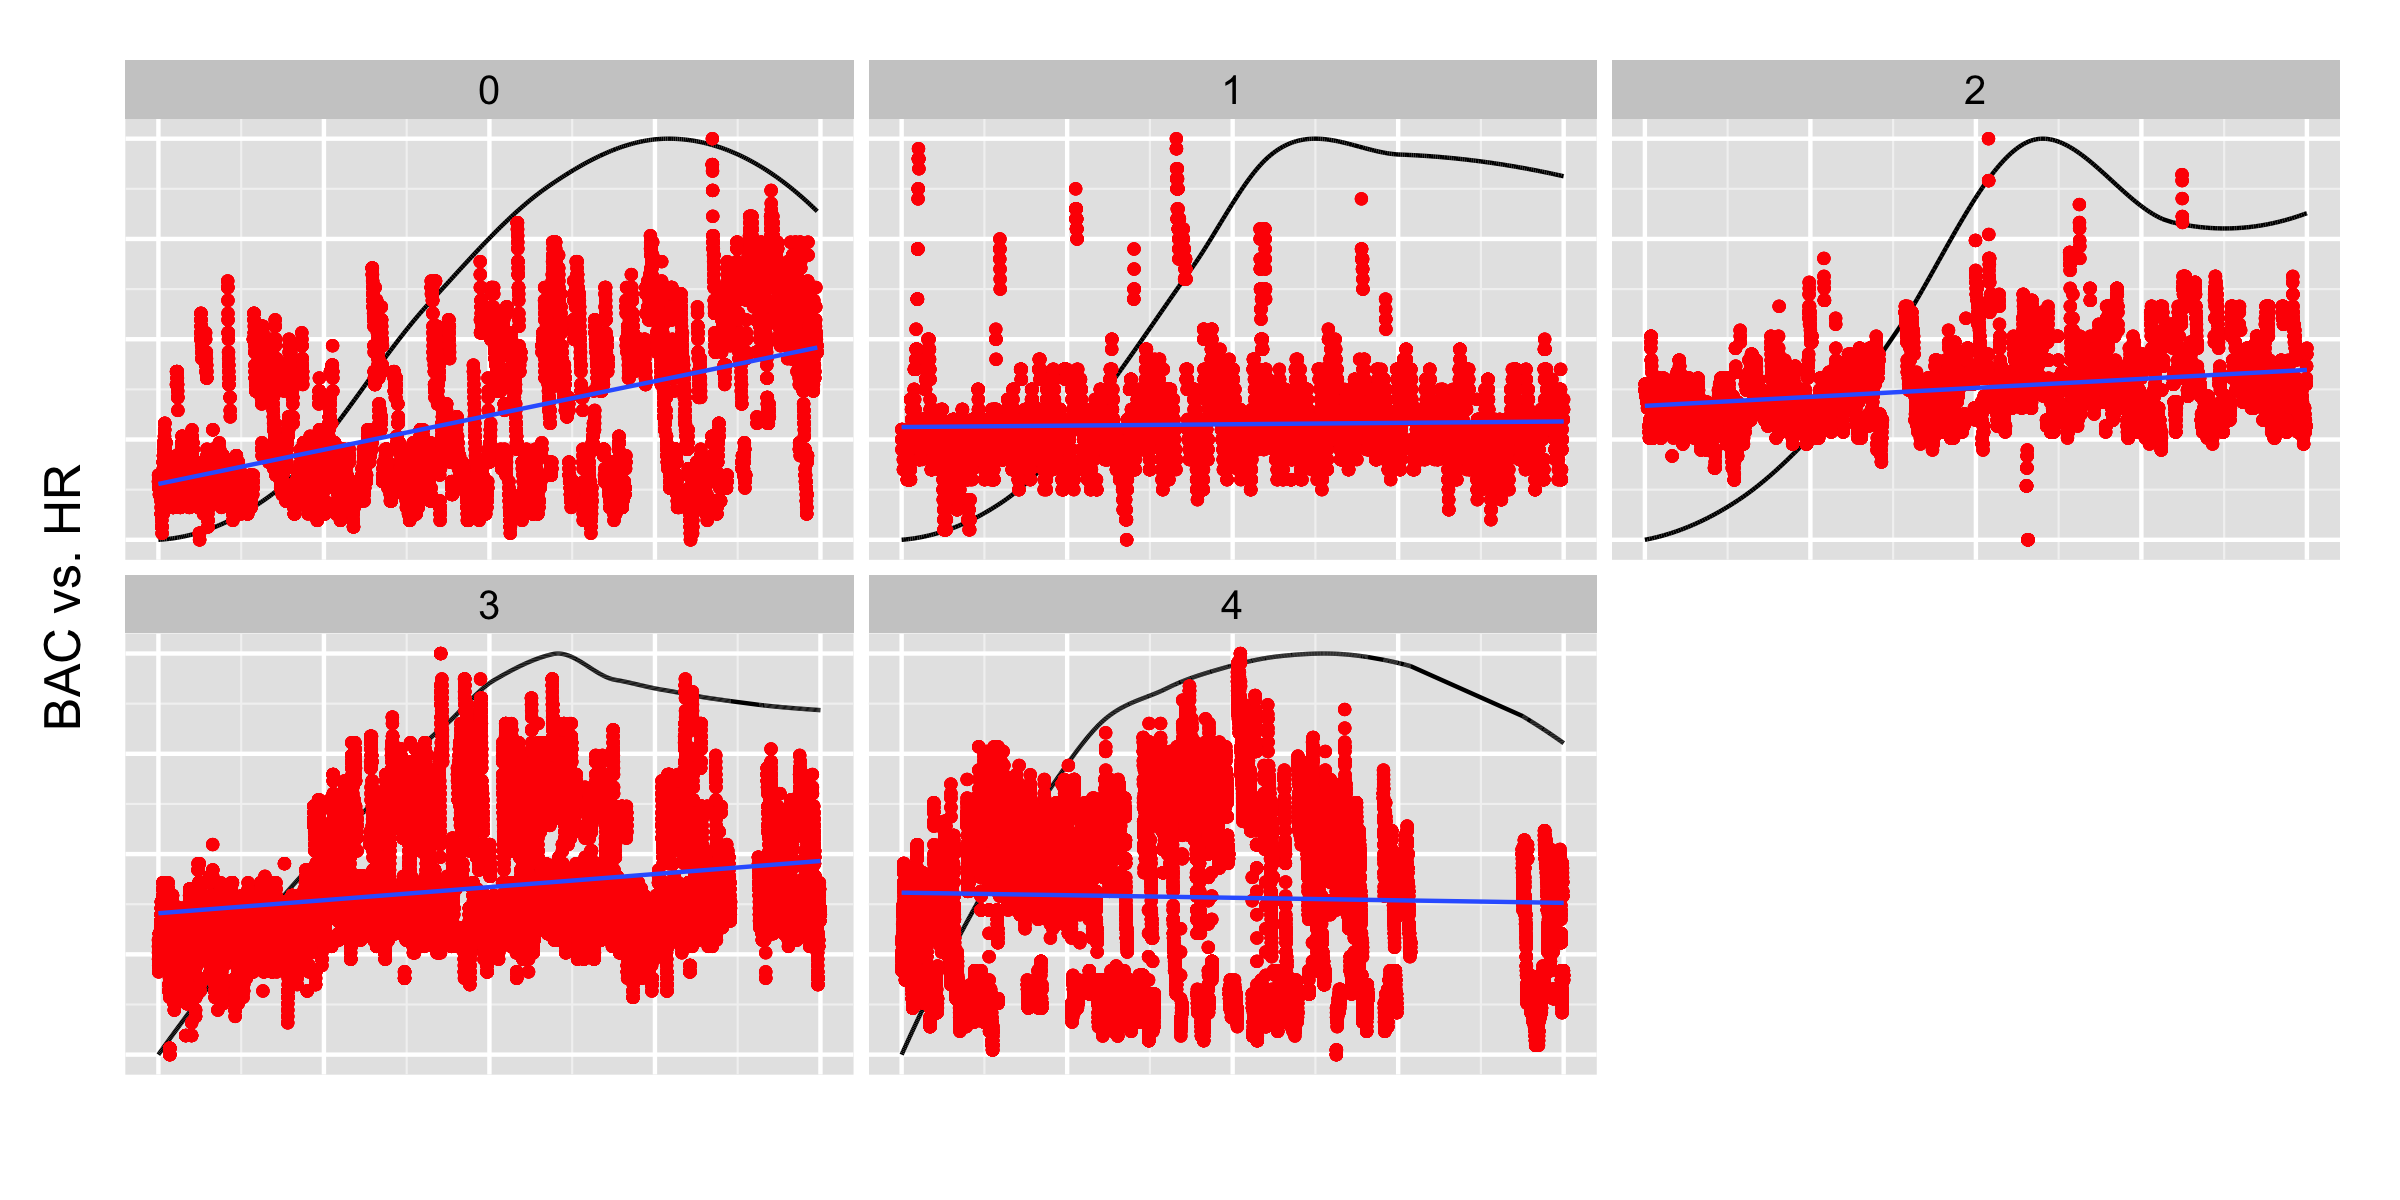
\includegraphics[width=1.0\textwidth]{../figs/heart_rates}
	\caption{Heart Rate and BAC per subject (normalized).}
	\label{fig:heart_rate_facet}
\end{figure}

The heart rate increases over time for three of the subjects (0, 2, 3) at different rates, decreases for one (4), and stays level for one (1). These observations are consistent with data in \cite{Assaad:2006}; a study where the authors relate low and high HR responses to behavioral traits. Interestingly, most of the subjects seem to show two patterns of HR activity. One is the baseline HR activity, and another is an excitied HR activity that seems to have better correlation with BAC. This is most clearly seen in the plot for subject 0, shown in Figure \ref{fig:heart_rate_split}. It's not a consistent pattern, however. Subject 1 had a very level heart rate with spikes at the regular drinking intervals, and subject 2 had relatively little variance throughout. Overall, it seems that experiencing excitement while intoxicated results in a more exaggerated HR response than while sober. This may be useful information for determining drunkenness.

\begin{figure}
	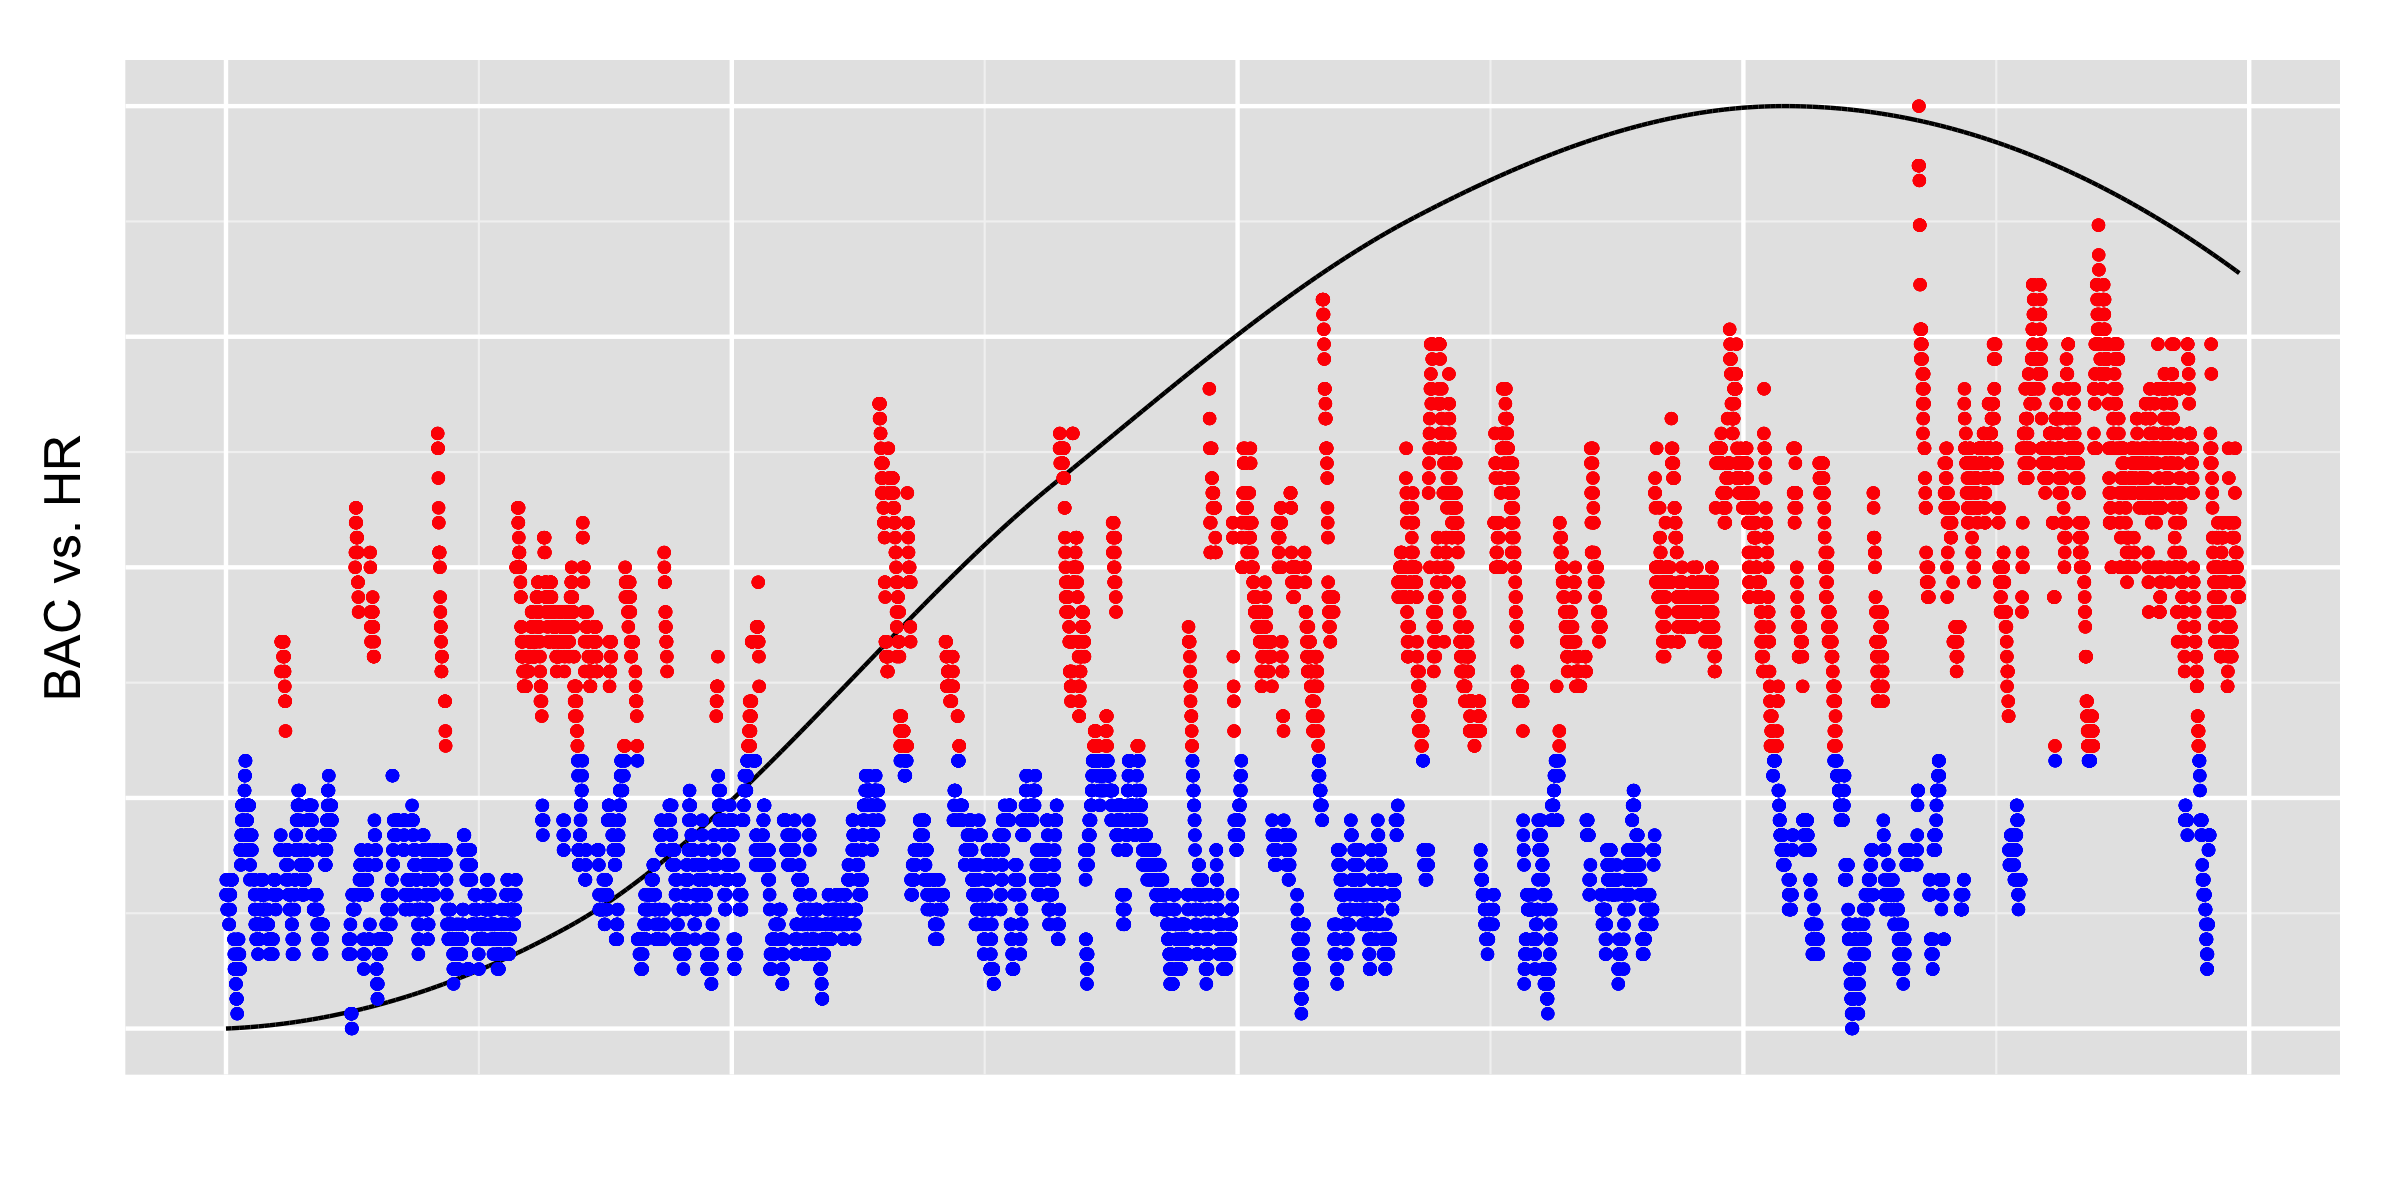
\includegraphics[width=1.0\textwidth]{../figs/heart_rate_split}
	\caption{Heart rate split into baseline and excited states.}
	\label{fig:heart_rate_split}
\end{figure}

Next, we plotted the normalized skin temperature over time on top of the normalized BAC values; this is shown in Figure \ref{fig:skin_temperatures}. Visually, we see that the correlation of skin temperature and BAC is highly significant. This is because of the well known vasodilation effect of alcohol causing warm blood to come near the surface of the skin \cite{Dekker:1999}. It is also known that with a high enough level of intoxication it behaves as a vasoconstrictor and drops skin temperature, which we see with subjects 4 and 5 who had reached the highest BAC of the group. Subject 2 had a rapid decrease in temperature at the beginning (we may have started collection too soon before the smartwatch sensor adjusted to his skin temperature), it may be appropriate to discard this portion.

\begin{figure}
	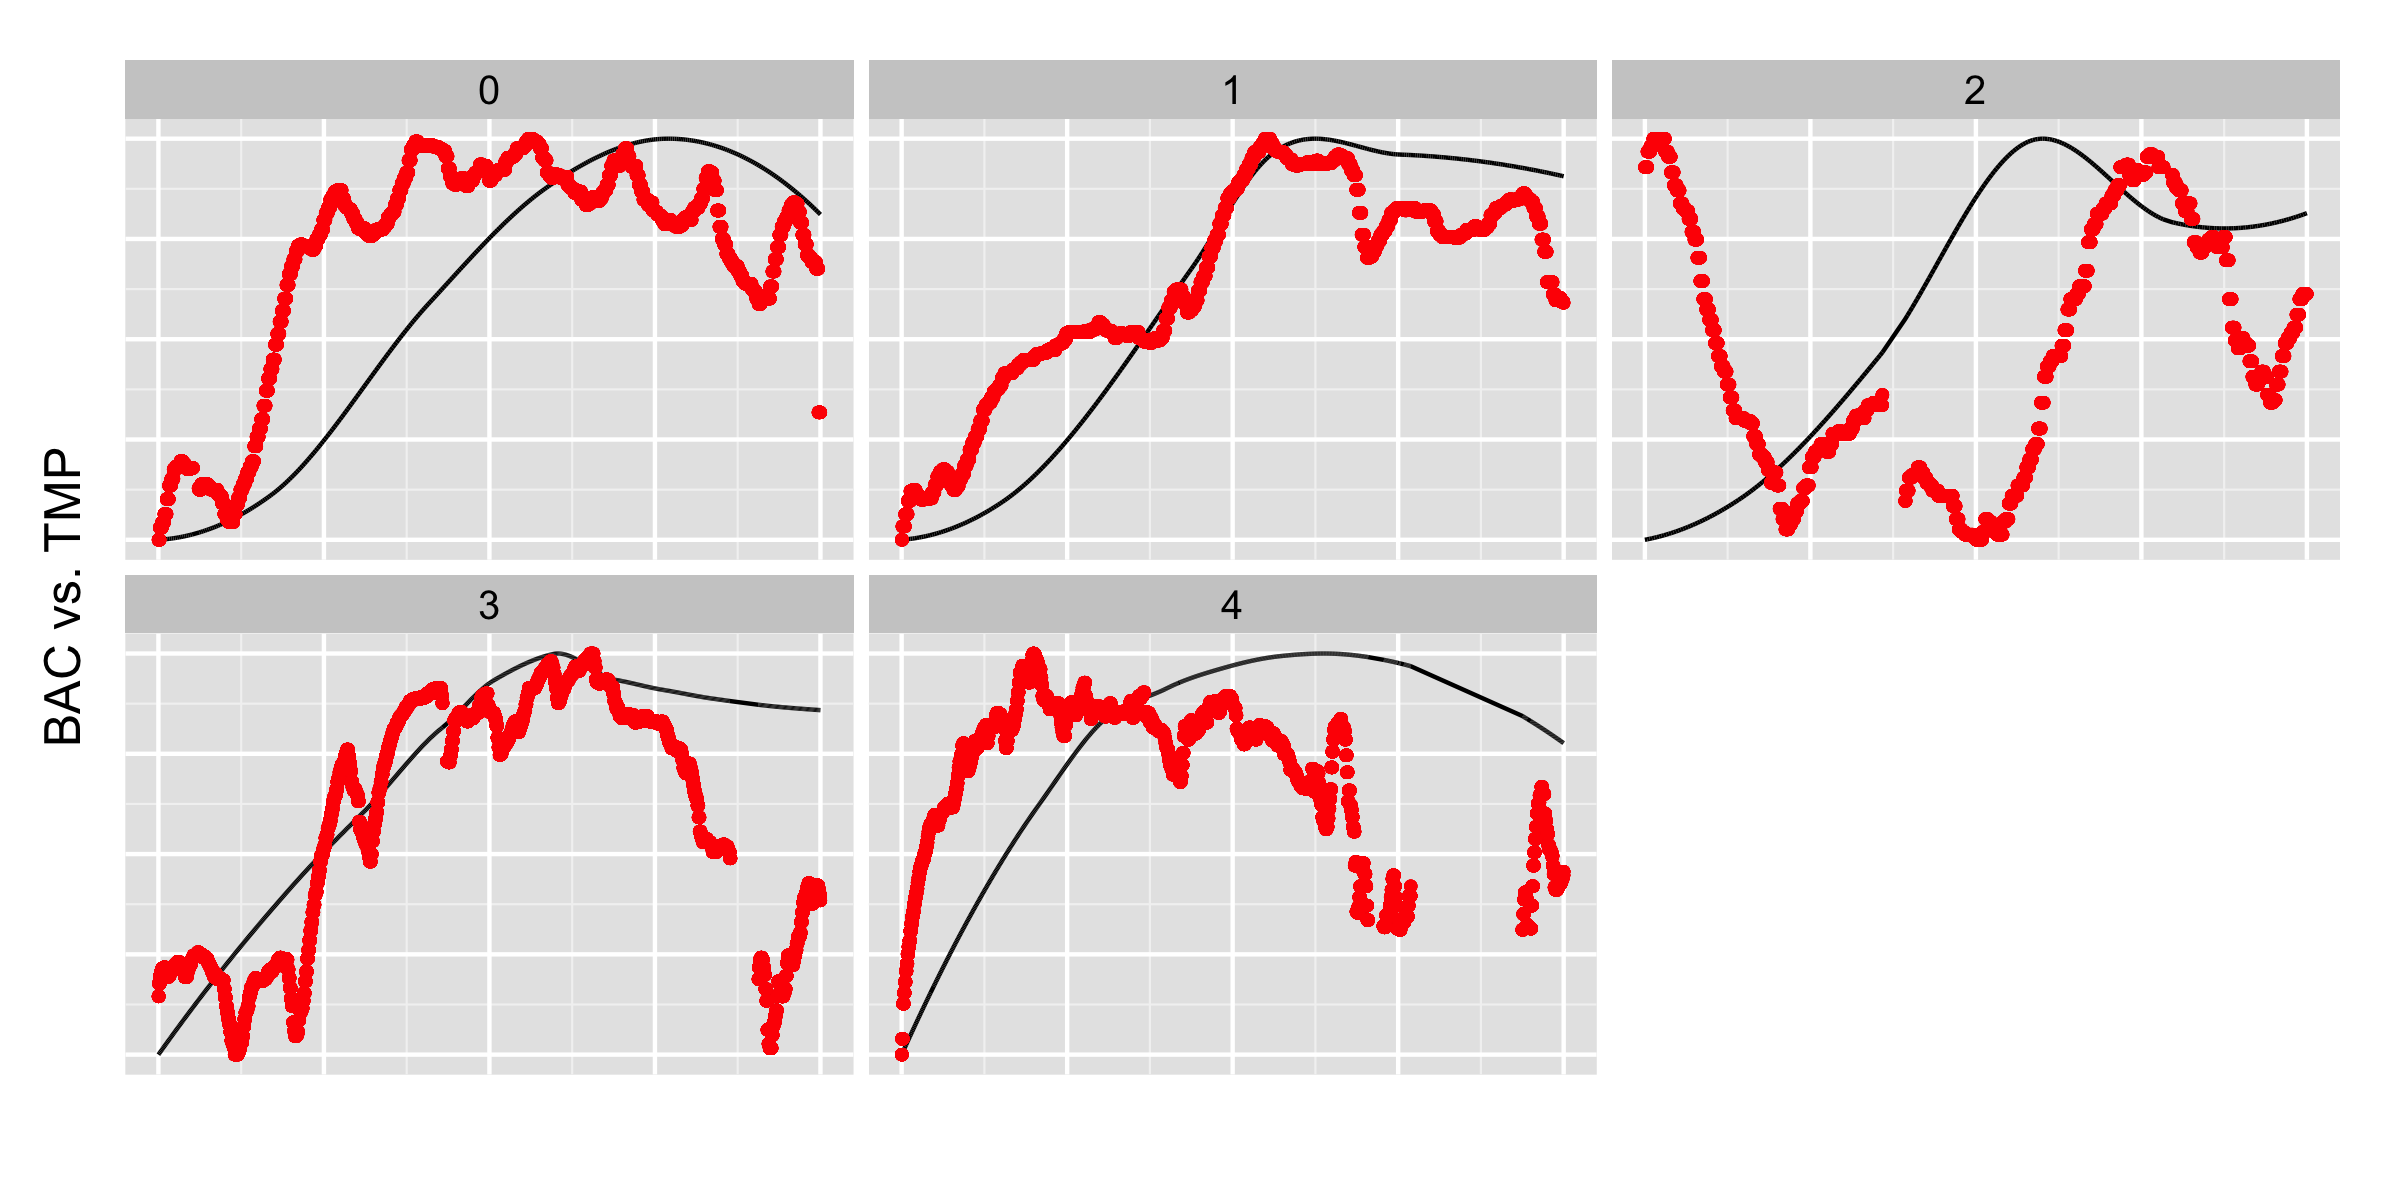
\includegraphics[width=1.0\textwidth]{../figs/skin_temperatures}
	\caption{Skin Temperature and BAC per subject (normalized).}
	\label{fig:skin_temperatures}
\end{figure}

The movement sensors (accelerometer and gyroscope) were not too interesting visually or statistically. They might have some hidden patterns that contribute to the performance of a modeling technique. We think it's usefulness will be increased if we can use it first to predict whether a user is taking a drink, then provide a time-based aggregate of the estimated number of drinks as a feature in our model to determine drunkenness.

\subsection{Features Setup}

Skin temperature and heart rate will have different ranges of values unique to each subject, so per-subject normalization must be performed to put them on the same scale. A simple unity-based normalization (min-max) is used to put the feature values in the range 0 to 1. No transformations are applied to the movement data.

\subsection{Models and Tools}

We will be taking a look at BAC prediction as both a classification and regression problem. As a classification problem, we will threshold the BAC values at a point where we may want to warn the user. This allows the data to be used as a binary classification problem. For this we will use: logistic regression, decision trees, and kNN. 

As a regression problem, we will be attempting to predict the observed BAC directly. To do this, we will use linear regression and neural networks. Using a regression approach, this will allow a user to select their own threshold rather than the threshold determined in a classification model. We may however want the threshold to be fixed.

All work will be performed in R version 3.2.1 using the 'caret' package. Specifics of the tuning parameters and setup will be described in the evaluation for each model along with the results. The evaluation metrics will include standard classification performance measures, such as: specificity, AUC, and F-score; along with RMSE for the regression models. Reported scores will be the mean cross-validation score to get a better idea of model performance on unseen data.
\section{Evaluation}

Overall, our data set contains 233,538 samples that were collected from five volunteers. Each sample was collected every three seconds from a Microsoft Band smartwatch by our Android data collection system. In this section, we evaluate the performance of a few machine learning models on our dataset. We use some standard performance measures for our evaluation: precision, recall, and F1-score, for the classification models; RMSE and R$^2$ for the regression models. All reported performance values are determined via 5-fold cross-validation.

\subsection{Classification}

We want to warn a person if they are close to reaching the legal limit of 0.08 BAC. A good time to warn a user is at about 0.065 BAC. Using this threshold, the classes are split into 64\% is \textit{DRUNK}, and 36\% \textit{SOBER}.

To get a baseline, we first trained a logistic regression model. This model outputs values from 0.0 to 1.0, so we need to determine where to best split this output into each class. In Figure \ref{fig:log_pred_density}, we show a plot of the predictions of the model on the test data, using the actual labels to distinguish the output. \begin{figure}
	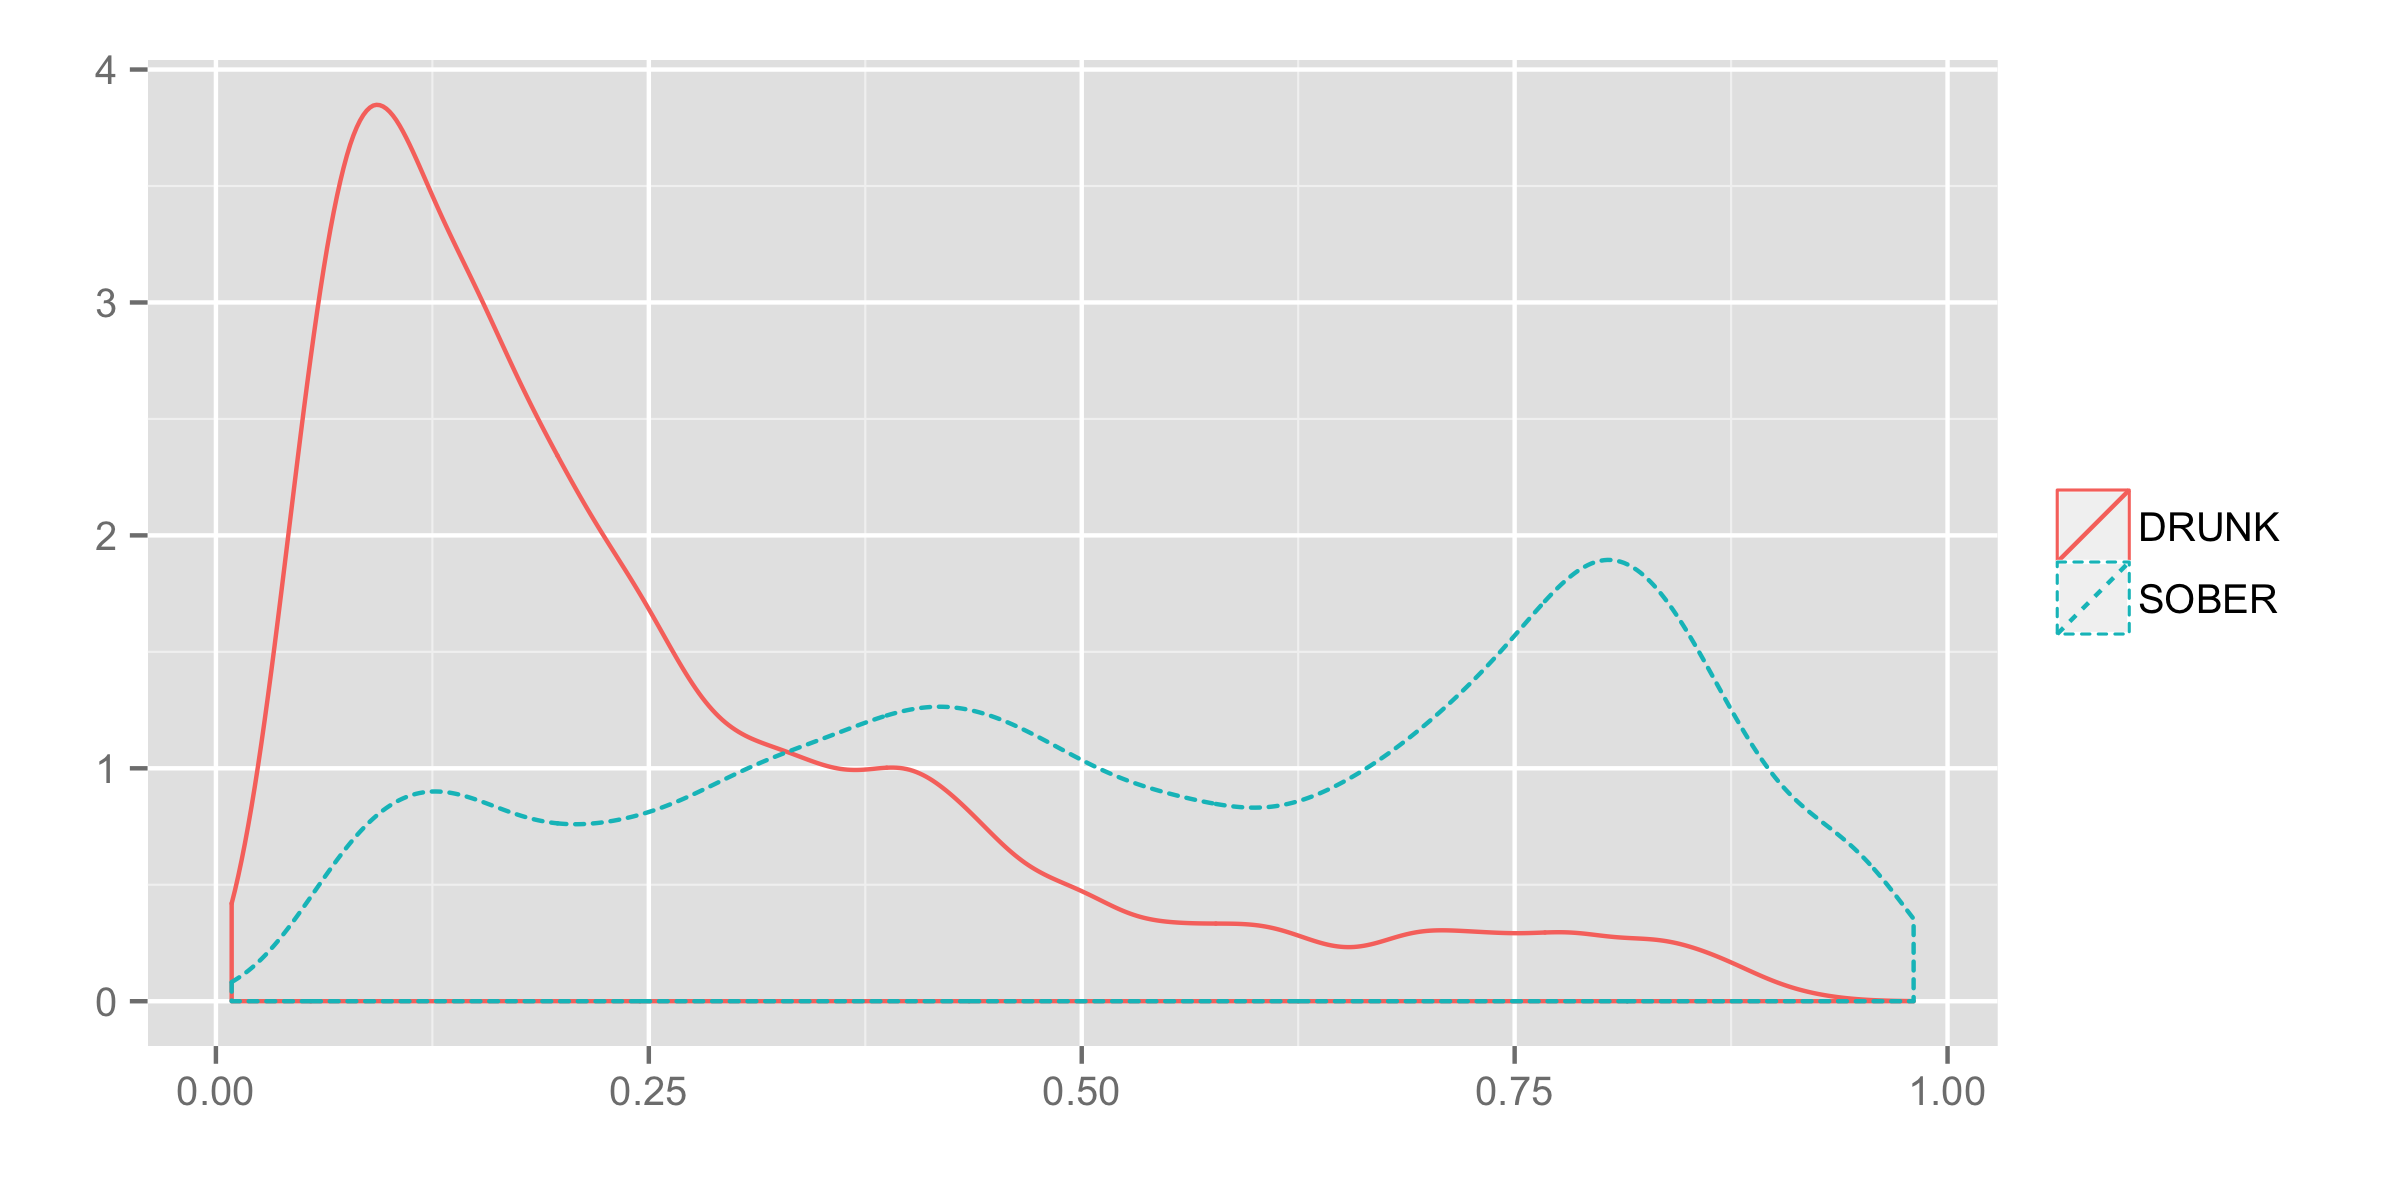
\includegraphics[width=1.0\textwidth]{figs/log_pred_density}
	\caption{Logistic regression output frequency with actual labels}
	\label{fig:log_pred_density}
\end{figure}In this plot, we see that the best threshold value for the logistic model predictions is around 0.32; above that we classify \textit{SOBER} and below that \textit{DRUNK}. Using this, we achieved a precision of 0.855 $\pm$ 0.002, recall of 0.730 $\pm$ 0.004, and F1-score of 0.787 $\pm$ 0.003.

Moving forward, we trained a SVM model using the Gaussian Radial Basis Function (RBF) kernel. For time constraints, the dataset was reduced by half using a uniform subsample. Even so, we found the SVM was able to achieve great performance with a precision of 0.886 $\pm$ 0.002, recall of 0.930 $\pm$ 0.002, and overall F1-score of 0.907 $\pm$ 0.001. Ideally we do not want to warn our users that they are drunk when they are not actually drunk, so we want to try and optimize the model to be as precise as possible. By modifying the error weighting to train against false positive errors, the SVM model achieved a precision of 0.970 $\pm$ 0.002, with recall of 0.729 $\pm$ 0.003, and F1-score of 0.832 $\pm$ 0.002. Our recall dropped for a higher precision, which is a well-known tradeoff for this kind of tuning, but this is fine. We can set a threshold on our smartphone warning system that if at least a recall fraction of the samples from our smartwatch are classified as \textit{DRUNK}, then there is a precision chance that the user is actually at 0.065 BAC.

\subsection{Regression}

So how does this do as a regression problem? We first considered the most basic: a linear regression model. This did not perform well at all. We next trained a neural network (ANN) model on the data. \begin{figure}
	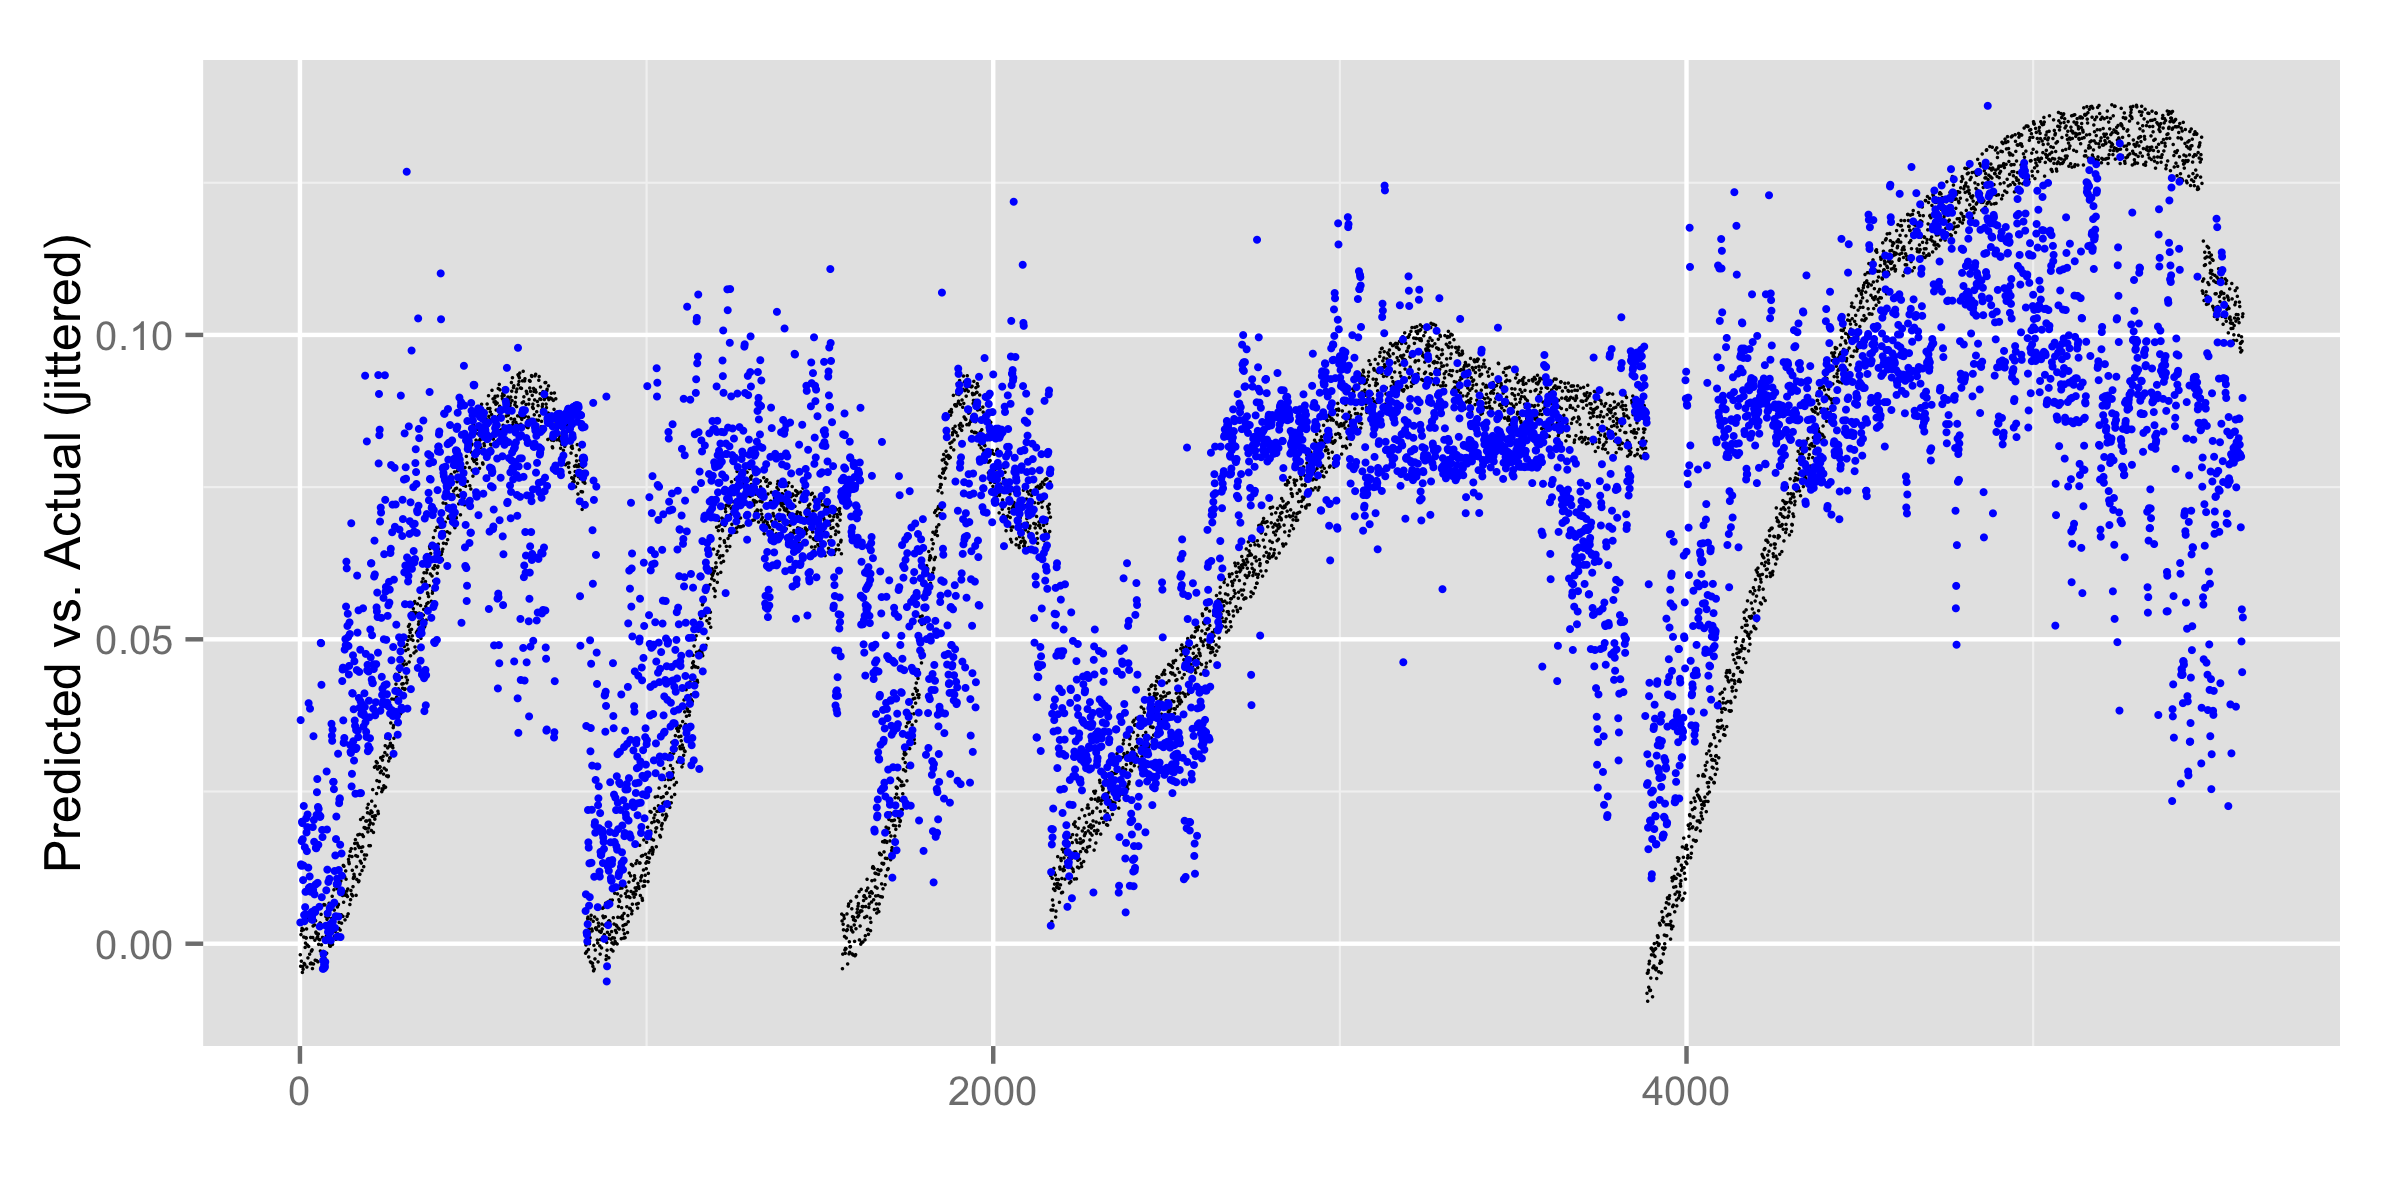
\includegraphics[width=1.0\textwidth]{figs/nn_all}
	\caption{ANN predictions (blue) with actual BAC data (black) on test partition}
	\label{fig:nn_all}
\end{figure}The best performing ANN had a structure with twenty nodes in one hidden layer. This was determined by doubling and then reducing node count to find the best performance. Additional layers did not show any improvement (the 'neuralnet' package was used to test multiple layers). Figure \ref{fig:nn_all} plots the BAC predictions of the ANN along with the actual values using data from a test partition. The ANN model achieved a R$^2$ value of 0.524 $\pm$ 0.015, with RMSE of 0.026 $\pm$ 0.000. It performed much better than the linear regression model, but not nearly as good as the classification models.
\section{Conclusions}

We investigated the design of a general system that could be used for many applications, whether it be a BAC warning system, or a geographical mapping service that displays the smartwatch data of users on a choropleth map. Part of this system was a general Android-based gateway that can be used to collect data from a variety of sensors connected to an Android smartphone.

We then designed an experiment to collect labeled data consistently from volunteers. After this, we analyzed the data to discover if there were any interesting patterns that were immediately obvious. We found that skin temperature was a good indicator of drunkenness (in our controlled setting). We also discovered that excited heart rate looks to also be a good indicator of intoxication level.

Following the overview analysis, we dove into training some regression and classification models. Achieving good performance as a regression problem was difficult. We found that the problem was much better tackled as a classification problem. This worked better because our classification models could ignore a good deal of the variance in the straight BAC predictions. In the end, we found SVM to perform the best on our data.

There are still many other factors to consider in forming a better models. From this research, we found that the accurate prediction of drunkenness in a real application looks possible in theory. There are still many obstacles surrounding the collection of a larger and better data set. Ideally, we would want a data set from a thousand volunteers in candid situations over several days. The two biggest problems are, how do we label the data with the alcohol levels in this scenario, and how can we model this enormous amount of data in reasonable time? Also, will we need to first determine the activity of the user, or will the other sensors provide sufficient information? And if the former, how can we consistently tag these activities in the data? The answers to this may be simple, or infeasible. In any case, it would be worth it to try and find out.
\subsection*{Acknowledgement}
We thank the National Science Foundation for funding the research under the Research Experiences for Undergraduates Program (CNS-1358939) at Texas State University to perform this piece of work and the infrastructure provided by a NSF-CRI 1305302 award.


% no keywords


% For peer review papers, you can put extra information on the cover
% page as needed:
% \ifCLASSOPTIONpeerreview
% \begin{center} \bfseries EDICS Category: 3-BBND \end{center}
% \fi
%
% For peerreview papers, this IEEEtran command inserts a page break and
% creates the second title. It will be ignored for other modes.
%\IEEEpeerreviewmaketitle


% An example of a floating figure using the graphicx package.
% Note that \label must occur AFTER (or within) \caption.
% For figures, \caption should occur after the \includegraphics.
% Note that IEEEtran v1.7 and later has special internal code that
% is designed to preserve the operation of \label within \caption
% even when the captionsoff option is in effect. However, because
% of issues like this, it may be the safest practice to put all your
% \label just after \caption rather than within \caption{}.
%
% Reminder: the "draftcls" or "draftclsnofoot", not "draft", class
% option should be used if it is desired that the figures are to be
% displayed while in draft mode.
%
%\begin{figure}[!t]
%\centering
%\includegraphics[width=2.5in]{myfigure}
% where an .eps filename suffix will be assumed under latex, 
% and a .pdf suffix will be assumed for pdflatex; or what has been declared
% via \DeclareGraphicsExtensions.
%\caption{Simulation Results}
%\label{fig_sim}
%\end{figure}

% Note that IEEE typically puts floats only at the top, even when this
% results in a large percentage of a column being occupied by floats.


% An example of a double column floating figure using two subfigures.
% (The subfig.sty package must be loaded for this to work.)
% The subfigure \label commands are set within each subfloat command, the
% \label for the overall figure must come after \caption.
% \hfil must be used as a separator to get equal spacing.
% The subfigure.sty package works much the same way, except \subfigure is
% used instead of \subfloat.
%
%\begin{figure*}[!t]
%\centerline{\subfloat[Case I]\includegraphics[width=2.5in]{subfigcase1}%
%\label{fig_first_case}}
%\hfil
%\subfloat[Case II]{\includegraphics[width=2.5in]{subfigcase2}%
%\label{fig_second_case}}}
%\caption{Simulation results}
%\label{fig_sim}
%\end{figure*}
%
% Note that often IEEE papers with subfigures do not employ subfigure
% captions (using the optional argument to \subfloat), but instead will
% reference/describe all of them (a), (b), etc., within the main caption.


% An example of a floating table. Note that, for IEEE style tables, the 
% \caption command should come BEFORE the table. Table text will default to
% \footnotesize as IEEE normally uses this smaller font for tables.
% The \label must come after \caption as always.
%
%\begin{table}[!t]
%% increase table row spacing, adjust to taste
%\renewcommand{\arraystretch}{1.3}
% if using array.sty, it might be a good idea to tweak the value of
% \extrarowheight as needed to properly center the text within the cells
%\caption{An Example of a Table}
%\label{table_example}
%\centering
%% Some packages, such as MDW tools, offer better commands for making tables
%% than the plain LaTeX2e tabular which is used here.
%\begin{tabular}{|c||c|}
%\hline
%One & Two\\
%\hline
%Three & Four\\
%\hline
%\end{tabular}
%\end{table}


% trigger a \newpage just before the given reference
% number - used to balance the columns on the last page
% adjust value as needed - may need to be readjusted if
% the document is modified later
%\IEEEtriggeratref{8}
% The "triggered" command can be changed if desired:
%\IEEEtriggercmd{\enlargethispage{-5in}}

% references section

% can use a bibliography generated by BibTeX as a .bbl file
% BibTeX documentation can be easily obtained at:
% http://www.ctan.org/tex-archive/biblio/bibtex/contrib/doc/
% The IEEEtran BibTeX style support page is at:
% http://www.michaelshell.org/tex/ieeetran/bibtex/
%\bibliographystyle{IEEEtran}
% argument is your BibTeX string definitions and bibliography database(s)
%\bibliography{IEEEabrv,../bib/paper}
%
% <OR> manually copy in the resultant .bbl file
% set second argument of \begin to the number of references
% (used to reserve space for the reference number labels box)
\bibliographystyle{../sty/splncs03}
\bibliography{references}


% that's all folks
\end{document}


